\documentclass[aspectratio=169, 14pt]{beamer}
\usepackage[utf8]{inputenc}
\usepackage[english]{babel}
\usepackage{tipa}
\usepackage{graphicx}
\usepackage{transparent}
\usepackage[ruled, lined, linesnumbered, commentsnumbered]{algorithm2e}
\usepackage{pgfplots}
\usepackage{tikz}
\usetikzlibrary{matrix,backgrounds}
\usetikzlibrary{arrows}
\usetikzlibrary {arrows.meta}
\usetikzlibrary{calc,shadows.blur,fit,positioning}
\usetikzlibrary{shapes.multipart,chains}
\usepackage{minted}
\usepackage{fontawesome5}
\usepackage{booktabs}
\usepackage{caption}
\usepackage{hyperref}
\hypersetup{
    colorlinks=true,
    linkcolor=blue,
    filecolor=magenta,      
    urlcolor=cyan,
    }
\urlstyle{same}
\usetheme{metropolis}
\metroset{block=fill}
\usecolortheme{default}
\definecolor{darkmidnightblue}{rgb}{0.0, 0.2, 0.4}
\definecolor{LightGray}{gray}{0.9}


%------------------------------------------------------------
%This block of code defines the information to appear in the
%Title page
\title[Data Structures] %optional
{Data Structures}

\subtitle{Linked Lists}

\author[CHEN Zhongpu] % (optional)
{CHEN Zhongpu}

\institute[] % (optional)
{
  School of Computing and Artificial Intelligence \\
  \href{mailto:zpchen@swufe.edu.cn}{zpchen@swufe.edu.cn}
}

\date[] % (optional)
{SWUFE, Fall 2022}

%End of title page configuration block
%------------------------------------------------------------


%------------------------------------------------------------
%The next block of commands puts the table of contents at the 
%beginning of each section and highlights the current section:

% \AtBeginSection[]
% {
%   \begin{frame}
%     \frametitle{Table of Contents}
%     \tableofcontents[currentsection]
%   \end{frame}
% }
%------------------------------------------------------------


\begin{document}

%The next statement creates the title page.
\frame{\titlepage}

%---------------------------------------------------------
%This block of code is for the table of contents after
%the title page
% \begin{frame}
% \frametitle{Table of Contents}
% \tableofcontents
% \end{frame}
%--------------------------------------------------------
\begin{frame}
\frametitle{A Small Quiz}
\begin{enumerate}
    \item A queue implements a LIFO policy.
    \item What does \texttt{[None] * 10} mean in Python?
    \item What is a \texttt{deque}?
\end{enumerate}
\end{frame}


\begin{frame}
    \frametitle{Task}
Try to explain what an \textbf{ADT} (abstract data type) is by searching on the Internet.
    

\end{frame}

{
    % \usebackgroundtemplate{\transparent{0.3}{\begin{picture}
    %     \includegraphics[height=0.7\paperheight]{cover}
    % \end{picture}    
    % }}
\usebackgroundtemplate{
  \tikz[overlay,remember picture] 
  \node[opacity=0.3, at=(current page.south east),anchor=south east, yshift=2cm,xshift=4cm] {
    \includegraphics[height=0.6\paperheight]{cover}};
}
    \begin{frame}
        \section{\textcolor{darkmidnightblue}{1. From List to ADT}}
    \end{frame}

}

\begin{frame}
    \frametitle{1.1 List}

\begin{exampleblock}{List}
An ordered collection (also known as a sequence).
\end{exampleblock} 

\begin{itemize}
    \item \texttt{add(e)}
    \item \texttt{get(i)}
    \item \texttt{remove(i)}
    \item \texttt{size()}
    \item ...
\end{itemize}
\pause
For users, they only care about what operations can be performed, but not \textbf{how these operations will be implemented}.

\end{frame}

\begin{frame}

    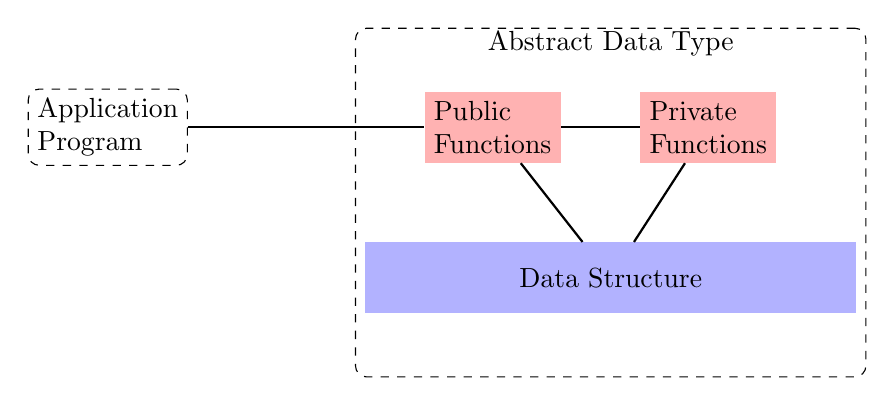
\begin{tikzpicture}[slot/.style={minimum size=0.9cm,rectangle}, data/.style={slot, fill=black!30}, 
        data2/.style={slot, fill=red!30},data3/.style={slot, fill=blue!30, align=center, text width=6cm}, >=Stealth]

        \node[draw, rounded corners, dashed, align=left](app){Application\\Program};

        \node[data2, align=left, right=of app, xshift=2cm] (public){Public\\Functions};
        \node[data2, align=left, right=of public](private){Private\\Functions};
        \node[data3, below=of public, xshift=1.5cm](data){Data Structure};

        \node [draw, rounded corners, inner ysep=.8cm, dashed, 
        fit=(public) (private) (data), label={[anchor=north, inner sep=1pt]north:Abstract Data Type}]{};

        \draw[thick] (app) -- (public);
        \draw[thick] (public) -- (private);
        \draw[thick] (public) -- (data);
        \draw[thick] (private) -- (data);
        
    \end{tikzpicture}


    \begin{quote}
    An abstract data type (\alert{ADT}) is a class (or type) of objects whose logical behavior is defined by a set of values and \underline{a set of operations}.
\end{quote}

\end{frame}

\begin{frame}
    \frametitle{Benefits of ADTs}
A \texttt{list/stack/queue/deque} is an \textbf{ADT}.
\begin{itemize}
    \item Code is easier to understand (e.g., it is easier to see high-level steps being performed, not obscured by low-level code).
    \item Implementations of ADTs can be changed (e.g., for efficiency) without requiring changes to the program that uses the ADTs.
    \item ADTs can be reused in future programs.
\end{itemize}

\end{frame}

\begin{frame}[fragile]
    \frametitle{1.2 Revisit List}
\texttt{ArrayList} in Java and \texttt{list} in Python are both based on \textbf{arrays}. Therefore, the elements are occupying \textbf{continuous} memories.

    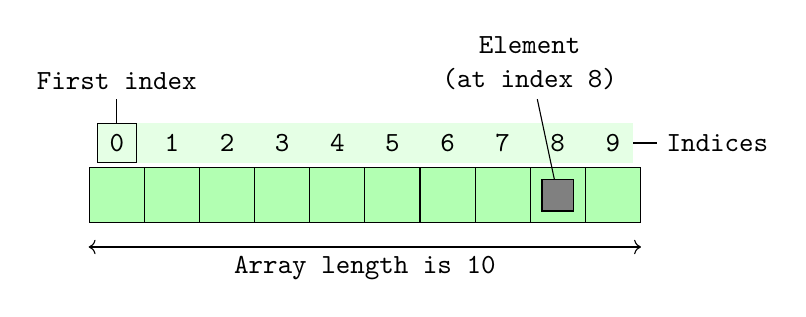
\begin{tikzpicture}[font=\ttfamily,
        array/.style={matrix of nodes,nodes={draw, minimum size=7mm, fill=green!30},column sep=-\pgflinewidth, row sep=0.5mm, nodes in empty cells,
        row 1/.style={nodes={draw=none, fill=none, minimum size=5mm}},
        row 1 column 1/.style={nodes={draw}}}]
        
        \matrix[array] (array) {
        0 & 1 & 2 & 3 & 4 & 5 & 6 & 7 & 8 & 9\\
          &   &   &   &   &   &   &   &   &  \\};
        \node[draw, fill=gray, minimum size=4mm] at (array-2-9) (box) {};
        
        \begin{scope}[on background layer]
        \fill[green!10] (array-1-1.north west) rectangle (array-1-10.south east);
        \end{scope}
        
        \draw[<->]([yshift=-3mm]array-2-1.south west) -- node[below] {Array length is 10} ([yshift=-3mm]array-2-10.south east);
        
        \draw (array-1-1.north)--++(90:3mm) node [above] (first) {First index};
        \draw (array-1-10.east)--++(0:3mm) node [right]{Indices};
        \node [align=center, anchor=south] at (array-2-9.north west|-first.south) (8) {Element\\ (at index 8)};
        \draw (8)--(box);
    \end{tikzpicture}
    

\end{frame}

\begin{frame}[fragile]

    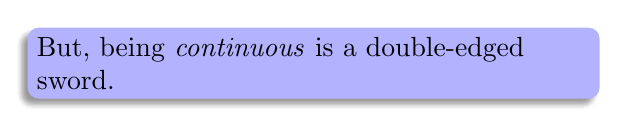
\begin{tikzpicture}
        \node[fill=blue!30,blur shadow={shadow xshift=-0.5ex},
        text width=20em,anchor=south west,rounded corners]
        {But, being \emph{continuous} is a double-edged sword.};
    \end{tikzpicture}

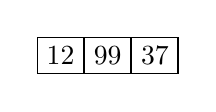
\begin{tikzpicture}
  \matrix[nodes=draw]
  {
    \node {12}; &
    \node {99}; &
    \node {37}; \\
  };
\end{tikzpicture}

\begin{itemize}
    \item Efficient in many index-based operations (e.g., \texttt{get(i)}).
    \item Inefficient while shifting or copying (e.g., removing the 1st element).
\end{itemize}

\pause

As for the List ADT, there is yet another implementation, named \alert{linked lists}, which are not \emph{continuous} in the memory.
    
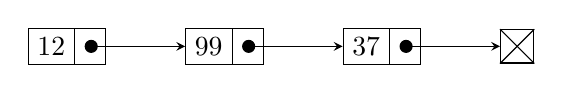
\begin{tikzpicture}[list/.style={rectangle split, rectangle split parts=2,
    draw, rectangle split horizontal}, >=stealth, start chain]

  \node[list,on chain] (A) {12};
  \node[list,on chain] (B) {99};
  \node[list,on chain] (C) {37};
  \node[on chain,draw,inner sep=6pt] (D) {};
  \draw (D.north east) -- (D.south west);
  \draw (D.north west) -- (D.south east);
  \draw[*->] let \p1 = (A.two), \p2 = (A.center) in (\x1,\y2) -- (B);
  \draw[*->] let \p1 = (B.two), \p2 = (B.center) in (\x1,\y2) -- (C);
  \draw[*->] let \p1 = (C.two), \p2 = (C.center) in (\x1,\y2) -- (D);
\end{tikzpicture}

\end{frame}

\begin{frame}

    \section{\textcolor{darkmidnightblue}{2. Linked Lists}} 

    \begin{quote}
        A linked list is a data structure in which the objects are arranged in a linear order, and the order in a linked list is determined by a pointer in each object.
    \end{quote}

\end{frame}

\begin{frame}
    \frametitle{2.1 Definition}

    \begin{columns}
        \column{.5\textwidth}
        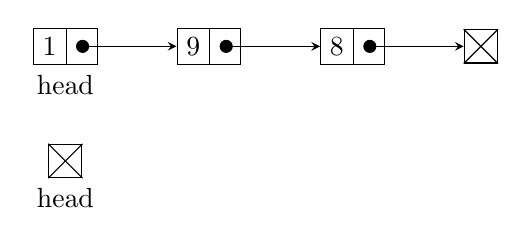
\begin{tikzpicture}[list/.style={rectangle split, rectangle split parts=2,
            draw, rectangle split horizontal}, >=stealth, start chain]
        
          \node[list,on chain] (A) {1};
          \node[list,on chain] (B) {9};
          \node[list,on chain] (C) {8};
          \node[on chain,draw,inner sep=6pt] (D) {};
          \draw (D.north east) -- (D.south west);
          \draw (D.north west) -- (D.south east);
          \draw[*->] let \p1 = (A.two), \p2 = (A.center) in (\x1,\y2) -- (B);
          \draw[*->] let \p1 = (B.two), \p2 = (B.center) in (\x1,\y2) -- (C);
          \draw[*->] let \p1 = (C.two), \p2 = (C.center) in (\x1,\y2) -- (D);
          \node[below=of A, yshift=1cm] (head){\alert{head}};
    
          \node[on chain,draw,inner sep=6pt, below=of A] (E) {};
          \draw (E.north east) -- (E.south west);
          \draw (E.north west) -- (E.south east);
    
          \node[below=of E, yshift=1cm] {\alert{head}};
        \end{tikzpicture}
        \column{.4\textwidth}
        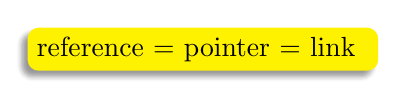
\begin{tikzpicture}
            \node[fill=yellow,blur shadow={shadow xshift=-0.5ex},
            text width=12em,anchor=south west,rounded corners]
            {reference = pointer = link};
        \end{tikzpicture}
    \end{columns}

    \begin{quote}
        A linked list is a \textbf{recursive} data structure that is either empty (null) or a reference to a node having an item and a reference to a linked list.
    \end{quote}

\end{frame}

\begin{frame}[fragile]
    \frametitle{2.2 Node in Python}

    \begin{minted}[bgcolor=LightGray]{python}
class Node:
    def __init__(self, item, next=None):
        self.item = item
        self.next = next

first = Node(1) # first is the head
second = Node(9)
third = Node(8)
first.next = second
second.next = third
    \end{minted}
\end{frame}

\end{document}